\documentclass[12pt]{report} % Times New Roman, 12pt
%\usepackage{gscale_thesis_singlespace} % Single spaced thesis
\usepackage{gscale_thesis_doublespace} % Double spaced thesis
\usepackage{fancyheadings} % Header and footer styling
\usepackage{natbib} % Bibliography formatting
\usepackage{setspace} % Allows double spacing but skips headers/footers
\setcounter{tocdepth}{1} % Limits the TOC to chapter and section names

% Additional packages
\usepackage{graphicx} % Allows the inclusion of figures
\usepackage{subcaption} % Allows captions to be added to subfigures
\usepackage[justification=centering]{caption} % Centres caption text
\usepackage{array} % Used for table formatting
\newcolumntype{P}[1]{>{\raggedright\let\newline\\\arraybackslash\hspace{0pt}}m{#1}}
\usepackage{booktabs} % Fancy-style tables
\usepackage{longtable} % Allows for tables that are more than one page long
\usepackage{float} % Better figure placement control
\usepackage{enumerate} % Numbered lists
\usepackage[shortlabels]{enumitem} % For controlling enumerate labels
\usepackage[shortcuts]{extdash} % Allows manual hyphenation of hypenated words
\usepackage{amsmath} % Non-standard math symbols
\usepackage{amsfonts} % Extended fonts for mathematics
\usepackage{listings} % Code section 
\usepackage{color} % Color setting
\usepackage[hidelinks]{hyperref} % Linking to LaTeX labels and external URLs

\numberwithin{equation}{section} % Numbers equations based on their section

\definecolor{lightgray}{gray}{0.96}
\definecolor{gray_ulisses}{gray}{0.55}
\definecolor{castanho_ulisses}{rgb}{0.71,0.33,0.14}
\definecolor{preto_ulisses}{rgb}{0.41,0.20,0.04}
\definecolor{green_ulises}{rgb}{0.2,0.75,0}

\lstdefinelanguage{HaskellUlisses} {
        frame=single,
        basicstyle=\ttfamily\footnotesize,
	sensitive=true,
        morecomment=[l][\color{gray_ulisses}\ttfamily]{--},
        morecomment=[s][\color{gray_ulisses}\ttfamily]{\{-}{-\}},
	morestring=[b]",
	stringstyle=\color{red},
	showstringspaces=false,
        numberblanklines=false,
	showspaces=false,
	breaklines=true,
	showtabs=false,
        backgroundcolor=\color{lightgray},
        emph=
        {[1]
		case,class,data,deriving,do,else,if,import,in,infixl,infixr,instance,let,
                module,of,primitive,then,type,where,foreign,import,export,ccall
        },
        emphstyle={[1]\color{blue}},
	emph=
	{[2]
        },
	emphstyle={[2]\color{castanho_ulisses}},
	emph=
	{[3]
        },
	emphstyle={[3]\color{preto_ulisses}\textbf},
	emph=
	{[4]
        },
	emphstyle={[4]\color{castanho_ulisses}\textbf},
	emph=
	{[5]
        },
	emphstyle={[5]\color{preto_ulisses}\textbf}
}

% ********************************
\begin{document}
\title{Your Thesis Title, Which Can Be As Long As You Want On the Title Page}
\halftitle{Short Title} % 60 Characters Max. Including Spaces

\author{Jane Doe}
\shortauthor{J. Doe} % Used for page header

\dept{Department You Belong To}
\field{Your Field} % What field your thesis is in (e.g. Software Engineering)

\prevdegreeone{B.Eng. (Software Engineering \& Game Design),\\ McMaster University, Hamilton, Canada}
\prevdegreetwo{B.Eng.} % Just your degree's field

\submitdate{MONTH YEAR} % Use the month's full spelling e.g. November
\copyrightyear{YYYY} % Year you are submitting this, usually your graduation 
%year

\doctype{Report} % ``Report'' or ``Thesis'' or whatever you need
\degree{Masters of Engineering} % The degree you get when you submit this
\degreeabbrv{M.Eng.}
\principaladviser{Your Supervisor} % Your Supervisor
 % LaTeX variables for preface pages/headers
    
\beforepreface % Half title page, title page, declaration page   
  \prefacesection{Lay Abstract}

A lay abstract of not more 150 words must be included explaining the key goals and contributions of the thesis in lay terms that is accessible to the general public.  % Lay Abstract
  \prefacesection{Abstract}
Drasil is a framework that generates software, including code, documentation, software requirement specification, user manual, and axillary files. Recently, the Drasil team has been interested in expanding its knowledge to solve higher-order ODEs. In this research, for single higher-order linear ODEs, the Drasil framework can solve them without manually extracted information. For higher-order nonlinear ODEs, the Drasil framework can solve them with manually extracted information.

Firstly, we design a flexible and reusable structure to store ODE information based on conventional mathematical knowledge. This makes it possible to reuse ODE information for documentation and for code generation. Secondly, we provide a commonality analysis of four external ODE solver libraries. The analysis includes how they solve the ODE, what algorithms they use, and what options they provide for different types of output. Thirdly, we enable the Drasil Code Generator to solve nonlinear higher-order ODEs with some manually extracted information. We created a new case study, Double Pendulum, that has a system of higher-order ODE. Further, we solve the Double Pendulum example numerically via external libraries. Lastly, for single higher-order ODEs, the Drasil Code Generator can generate code without manually extracted information.

This research accomplishes three main goals. Firstly, we capture the knowledge of linear ODE in a flexible and reusable structure. Secondly, we expand the Drasil capability to solve higher-order ODEs with/without manually written equations. Solving single higher-order linear ODEs does not require manually extracted information. To solve nonlinear ODEs, manually extracting information from the original ODE is still required. The last one is removing the duplicated information caused by the implementation of solving ODEs. % Abstract
  %\thispagestyle{empty}
\null\vfill
\begin{center}
%\textbf{Dedications}
%\linebreak
\textsl{Your Dedication \\ Optional second line}
\end{center}
\vfill
 % Dedication
  todo
 % Acknowledgements
  \referencepages % Table of Contents, List of Figures, List of Tables
  \prefacesection{Notation, Definitions, and Abbreviations}

\section*{Notation}
\begin{description}[font=\rmfamily\bfseries, leftmargin=3.5cm, style=nextline]
	\item[$\mathbb{R}$] any real number in (-$\infty$, $\infty$).
	\item[$\mathbb{R}^n$] a sequence that contains real numbers, n depends on number of inputs values.
	\item[$\mathbb{R}^i$] a finite sequence that contains real numbers, i depends on the start time, end time, and time step.
	\item[$\mathbb{R}^j$] a infinite sequence that contains real numbers, j is a natural number.
	\item[$\mathbb{R} \rightarrow \mathbb{R}^k$] a function takes an independent variable and outputs a sequence of dependent variables.
\end{description}

\section*{Definitions}
\begin{description}[font=\rmfamily\bfseries, leftmargin=5cm, style=nextline]
	\item[Drasil Framework] references the whole \href{https://jacquescarette.github.io/Drasil/}{Drasil Project}.
	\item[Drasil Code Generator] compile captured knowledge to code.
	\item[Drasil Printer] displays captured knowledge in SRS.
\end{description}

\section*{Abbreviations}
\begin{description}[font=\rmfamily\bfseries, leftmargin=3.5cm, style=nextline]
	\item[ACM] Apache Commons Maths
	\item[BDF] Differentiation Formula Method
	\item[BVP] Boundary Value Problem
	\item[DblPendulum] Double pendulum
	\item[GOOL] Generic Object-Oriented Language
	\item[IVP] Initial Value Problem
	\item[NoPCM] Solar water heating system without PCM
	\item[ODE] Ordinary differential equation
	\item[PDController] Proportional derivative controller
	\item[RK] Runge-Kutta
	\item[SCS] Scientific computing software
	\item[SglPendulum] Single Pendulum
	\item[SRS] Software requirements specification
\end{description}
  \academicstatement{academicachievementdeclaration}
\afterpreface
  
  
  \section{Problem Statement}

In Drasil, we are focused on understanding families of scientific software, and
creating systematic rules to generate families of software solutions (for any
instance of a scientific problem that requires a scientific software solution).
Specifically, Drasil is focused on mathematics and physics-based models. In both
areas, we are concerned with what \textit{kinds of theories} are
well-understood, and ensuring that all created mathematical expressions are
``valid''.

\intodo{Move above paragraph to the top of the ``Drasil'' section.}

\section{Contributions of the Author}

\begin{itemize}
      \item The problem of obtaining more information from our theories so that we
            may make better use from their meta-level information was understood
            before this work.
      \item A partial solution to this problem was also constructed before this
            work.
      \item The expression language used to build theories and, ultimately, inputs
            to outputs was constructed before this work.
\end{itemize}

\section{Thesis Outline}

In \autoref{chap:ideology}, we discuss the focal ideology underpinning this
work, and Drasil. \autoref{chap:drasil} describes Drasil, the host project
carrying the fruits of this work. \autoref{chap:modelkinds} discusses how
theories are encoded in Drasil, the issues associated with using a single
universal mathematical language to describe theories, and how we can resolve
these problems. \autoref{chap:typedExpr} describes residual issues associated
with validating and transcribing mathematical expressions.
\autoref{chap:knowledgeMgmt} continues to discuss the ways in which general
knowledge and theories are encoded in Drasil, and methods for altering their
encoding, leading into \autoref{chap:futureWork}, where we discuss future work.
                  
        \setcounter{figure}{0}
        \setcounter{equation}{0}
        \setcounter{table}{0}
        
  \chapter{ODE Data Representation}
In the Drasil framework, there is a single data structure containing all the information for all products, and we call it System Information. The giant System Information collects a multitude of pieces of information; whenever we need it, we extract the information from the System Information. In previous research, we store all ordinary differential equations (ODEs) information in the System Information. However, that information existed in the form of plain text. In other words, we explicitly wrote ODEs in the text without any advanced data structure. Although this method maintains the relationship of ODEs, it restricts any transformation of ODEs. For example, if the text-based ODE is higher-order linear ODE, we can not transform it to its equivalent system of first-order ODE. Therefore, the Drasil team is exploring new approach to store ODEs in a new data structure, and the new structure would allow ODEs be isomorphic, which means we can map the ODE from one form to other forms. Once we capture ODEs information in this data structure, we can generate its equivalent forms. This approach is contrasting to previous method, and it only requires users write ODEs once. This chapter we will discuss the problem occurs in text-based expression, introduce where the new data structure comes from, how the new data structure captures ODE information, how to use the new data structure, and how the new data structure interacts with the Drasil printer.

\section{Explicit Equation}
Before we conduct this research, the Drasil framework can generate software that provides numerical solutions for a first-order ODE by explicitly writing the equation. We re-write the ODE equation and pass it to the Drasil code generator. In Equation~\ref{eq_nopcmorginal}, the model describes the energy balance of water. In \href{https://jacquescarette.github.io/Drasil/examples/nopcm/SRS/srs/NoPCM_SRS.html#Sec:IMs}{NoPCM case study}, we can find the temperature of the water base on it.

\begin{equation} \label{eq_nopcmorginal}
	T_{w}'(t) +  \frac {T_{w}(t)}{\tau_{w}} = \frac{T_{c}}{\tau_{w}}
\end{equation}

The $T_w(t)$ is a function of the independent variable, in this case time. The $T_w$ is the temperature of water ($ ^\circ C $). The $T_w'(t)$ is the first directive of the function $T_w(t)$ respect time. The $T_c$ is the temperature of the heating coil (°C), and the $\tau_w$ is the ODE parameter for water related to decay time (s). We can later isolate the $T_w'(t)$ to the left-hand side and move the rest terms to the right-hand side. Then, we can get Equation~\ref{eq_nopcmderive}.
\begin{equation} \label{eq_nopcmderive}
	T_{w}'(t) = \frac{T_{c} - T_{w}(t)}{\tau_{w}}
\end{equation}

Based on Equation~\ref{eq_nopcmderive}, we can write it into a text-based form and pass it to the Drasil code generator. Code~\ref{code_expliciteq} shows how to encode Example~\ref{ex_firstorderode} by writing the explicit equation. Brooks's thesis~\citep{brooks} documented how the Drasil framework solves Equation~\ref{eq_nopcmderive} with manually created \href{https://jacquescarette.github.io/Drasil/docs/drasil-code-0.1.9.0/Language-Drasil-Code.html#t:ODEInfo}{ODEInfo}. The \verb|ODEInfo| is a data type holds ODE information. 

The user will first encode the ODE equation in the general data pool. Whenever we need it, we retrieve the ODE equation from it. However, there is a gap between the original equation and external libraries (Chapter~\ref{cha_extlib}). The external libraries can not understand the original ODE equation from the general data pool. Therefore, the Drasil team manually transforms the original ODE equation into another form (\verb|ODEInfo|), which external libraries can use to produce a numerical solution.

Here is an example of how we manually close the gap between the text-based ODE and external libraries. In Code~\ref{code_expliciteqsrs}, we encode Equation~\ref{eq_nopcmderive} and put it into the general data pool. During printing the SRS, we retrieve the text-based ODE and print it. The Drasil printer is capable of displaying encoded ODE in text. However, external libraries require a specific format for the ODE and can not utilize the original ODE. Therefore, we manually create Code \ref{code_expliciteq} so external libraries can solve the ODE. They both describe the same ODE, but we write it twice in the Drasil framework. Therefore, there is an information duplication. We can transform from Code~\ref{code_expliciteqsrs} to Code~\ref{code_expliciteq} with human interference. However, without human interference, we can not complete the transformation because Code~\ref{code_expliciteqsrs} lacks the necessary structure. To reduce the information duplication, the Drasil team decided to make an advanced data structure to hold the ODE information.

\begin{listing}[ht]
\begin{haskell1}
-- Pesodu Code
T_w'(t) = reciprocal τ_w * (T_c - T_w(t))
\end{haskell1}
\captionof{listing}{NoPCM equation for SRS}
\label{code_expliciteqsrs}
\end{listing}

\begin{listing}[ht]
\begin{haskell1}
-- Pesodu Code
reciprocal τ_w * (T_c - T_w[0])
\end{haskell1}
\captionof{listing}{NoPCM equation for the Drasil Code Generator}
\label{code_expliciteq}
\end{listing}

\section{Matrix Form}
In general, an equation contains a left-hand expression, a right-hand expression, and an equal sign. The left-hand and right-hand expressions connect by an equal sign. A linear ODE also has its left-hand and right-hand sides. Each side has its unique shape. We can write a linear ODE in the shape of

\begin{equation} \label{eq_matrixform}
	\boldsymbol{Ax} = \boldsymbol{b}
\end{equation}

On the left-hand side, \textbf{A} is an m $\times$ n matrix, and \textbf{x} is an n-vector. On the right-hand side, \textbf{b} is an m-vector. The \textbf{A} is commonly known as the coefficient matrix, \textbf{b} is the constant vector, and \textbf{x} is the unknown vector. The equation~\ref{eq_matrixform} can represent not only a single linear ODE, but also represent a linear system of ODE. A linear system of ODE is a finite set of linear differential equations. In this research, we only have case studies for single ODE, and all examples will demonstrate on single ODEs. The new data structure is capable to store information for a system of ODE, but its related functions only support for instances of single ODE.

Given the ODE example~\ref{eq_odeexmaple} in \href{https://jacquescarette.github.io/Drasil/examples/pdcontroller/SRS/srs/PDController_SRS.html#Sec:IMs}{PDContoller case study},
\begin{equation} \label{eq_odeexmaple}
	y_t''(t) + (1 + K_d) \cdot y_t'(t) + (20 + K_p) \cdot y_t(t) = r_t \cdot K_p
\end{equation}

In Example~\ref{eq_odeexmaple}, there is only one dependent variable $y_t$. The $y_t$(t) is a function of independent variable, in this case time. The $y_t'$(t) is the first derivative of $y_t$(t) respect time. The $y_t''$(t) is the second derivative of $y_t$(t) respect time. The $y_t$ is the process variable, and the $y_t'$ is the rate of change of $y_t$. The $y_t''$ is the rate of change of the rate of change of $y_t$. The $K_d$ , $K_p$, and $r_t$ are constant variables. The $K_d$ is Derivative Gain, $K_p$ is Proportional Gain, and $r_t$ is Set-Point. We can write this equation as follows.

\begin{equation} \label{eq_matrixformexmaple}
	\begin{bmatrix}
		1, & 1 + K_{d}, & 20 + K_{p}
	\end{bmatrix}
	\cdot
	\begin{bmatrix}
		y_{t}''(t)  \\
		y_{t}'(t)   \\
		y_{t}(t)  
	\end{bmatrix}
	=
	\begin{bmatrix}
		r_{t} \cdot K_{p} 
	\end{bmatrix}
\end{equation}

The relationship between the matrix form~\ref{eq_matrixform} and the example~\ref{eq_matrixformexmaple} is not hard to find. Firstly, the coefficient matrix \textbf{A} is a 1 $\times$ 3 matrix that consists of $1$, $1 + K_d$, ane $20 + K_p$. Secondly, the unknown vector \textbf{x} is a 3 $\times$ 1 vector with $y_t''$, $y_t'$, and $y_t$. Last, the constant vector \textbf{b} is a 1 $\times$ 1 vector with $r_t \cdot K_p$. The matrix form~\ref{eq_matrixform} very well captures all the knowledge we need to present an ODE. But, how a matrix form looks like in a nth-order linear ODE? Based on Paul's Online Notes~\citep{paullinearode}, we can write all linear ODEs in the shape of

\begin{equation} \label{eq_linearDE}
	a_n(t) \cdot y^n(t) + a_{n-1}(t) \cdot y^{n-1}(t) + \dots + a_1(t) \cdot y'(t) + a_0(t) \cdot y(t) = h(t)
\end{equation}

The coefficient $a_0(t), \dots, a_n(t)$ and $g(t)$ can be constant or non-constant functions, in our case they are constant functions. We also can write Equation~\ref{eq_linearDE} in a matrix form.

\begin{equation} \label{eq_matrixnthorder}
	\begin{bmatrix}
		a_n(t), & a_{n-1}, \dots, & a_0(t)
	\end{bmatrix}
	\cdot
	\begin{bmatrix}
		y_{t}^{n}(t) \\
		y_{t}^{n-1}(t) \\
		\dots \\
		y_{t}(t)  
	\end{bmatrix}
	=
	\begin{bmatrix}
		h(t)
	\end{bmatrix}
\end{equation}

Therefore, we decided to create a datatype called \verb|DifferentialModel| to preserve ODEs information. The \verb|DifferentialModel| has six records, and here is the representing code for \verb|DifferentialModel|.
\begin{haskell1}
data DifferentialModel = SystemOfLinearODEs {
	_indepVar :: UnitalChunk,
	_depVar :: ConstrConcept,
	_coefficients :: [[Expr]],
	_unknowns :: [Unknown],
	_dmConstants :: [Expr],
	_dmconc :: ConceptChunk
}
\end{haskell1}

Previous to this research, UnitalChunk, ConstrConcept, Expr, and ConceptChunk already existed in Drasil. We created an \verb|Unknown| type for this experiment. Their semantics will show up in table ~\ref{tab_demodeltype}

\begin{table}[ht]
	\begin{tabular}{ p{0.2\textwidth} p{0.7\textwidth} }
		\textbf{Type} & \textbf{Semantics} \\
		\toprule
		\verb|UnitalChunk| & concepts with quantities that must have a unit definition.\\
		\verb|ConstrConcept| & conceptual symbolic quantities with Constraints and maybe a reasonable value.\\
		\verb|Expr| & a type encode mathematical expression. \\
		\verb|ConceptChunk| & a concept that contains an idea, a definition, and an associated domain of knowledge\\
        \verb|Unknown|& synonym of Integer\\
		\bottomrule	
	\end{tabular}	
	\caption{Type use in DifferentialModel}	
	\label{tab_demodeltype}
\end{table}

The \verb|_indepVar| represents the independent variable, and it is often time. The \verb|_depVar| represents the dependent variable. Combing \verb|_depVar| and \verb|_indepVar|, it represents a function produce dependent variables over time. The \verb|_coefficients| is a list of lists \verb|Expr|, and it represents the coefficient matrix \textbf{A}. The \verb|_unknowns| is a list of \verb|Unknown|, and \verb|Unknown| is synonym of integers.
The \verb|_unknowns| represent a list of numbers of derivatives of the function. Combining \verb|_depVar|, \verb|_indepVar| and \verb|_unknowns|, they can represent the unknown vector \textbf{x}. The \verb|_dmConstants| is a list of \verb|Expr|, and it represents the constant vector \textbf{b}. Last, the \verb|_dmconc| contains metadata of this model. To represent example~\ref{eq_odeexmaple} in \verb|DifferentialModel|, \verb|_indepVar| is time, \verb|_depVar| is $y_t$, \verb|_coefficients| is the 1 $\times$ 3 matrix, \verb|_unknowns| is the 3 $\times$ 1 vector, \verb|_dmConstants| is the 1 $\times$ 1 vector, and \verb|_dmconc| is \verb|ConceptChunk| that describes what this model is. Code~\ref{code_interaldata} shows the internal data representation of the example~\ref{eq_odeexmaple} in \verb|DifferentialModel|.

\begin{listing}[ht]
\begin{haskell1}
_indepVar = time
_depVar = y_t
_coefficients = [[1, 1 + K_d, 20 + K_p]]
_unknowns = [2, 1, 0]
_dmConstants = [r_t * K_p]
_dmconc = ... -- Drasil definition for chuck concept
\end{haskell1}
\captionof{listing}{Internal Data Representation for Example~\ref{eq_odeexmaple}}
\label{code_interaldata}
\end{listing}

Currently, the \verb|DifferentialModel| only captures the knowledge of ODEs with one dependent variable, and it is a special case of the family of linear ODEs. Studying this special case will help the Drasil team better understand how to capture the knowledge of all ODEs and eventually lead to solving a system of linear ODE with multiple dependent variables. On top of that, there is one assumption. The \verb|_coefficients| can only be functions of independent variable, often time. In other word, the \verb|_coefficients| does not depend on \verb|_depVar|.

\section{Input Language}
\label{sec_input}
There are many reasons why we want to provide an input language for users to input ODE equations. One major reason is that it could be over complicated for users to input a single ODE in a matrix form. While inputting a single ODE, one obvious way is directly passing value to each record via constructors of \verb|DifferentialModel|. The Code~\ref{code_interaldata} shows how to encode Example~\ref{eq_odeexmaple} in the \verb|DifferentialModel|. However, it would be not so elegant to set a single ODE in the example, because users have to extracts the coefficient matrix \textbf{A}, unknown vector \textbf{x} and constant vector \textbf{b} from the original equation manually. Once the coefficient matrix, unknown vector and constant vector is ready, we can set value into \verb|_depVar|, \verb|_coefficients|, \verb|_unknowns|, and \verb|_dmConstants| accordingly. This process is ideal when the ODE is a system of ODE, and it would be over-complicated for user to do extraction for a single ODE. Therefore, we decided create a helper function to ease this issue. On top of that, the Drasil printer will print a single ODE in SRS with a more familiar ``one line equation'' form. Another advantage of having an helper function to input an ODE is that it can reduce human error and make sure the equation is well-formed. We call this helper function input language, and what will this input language looks like? 

The input language is inspired by how a linear nth-order ODE looks like. Based on Paul's Online Notes~\citep{paullinearode}, we can write all linear ODEs in the shape of Equation~\ref{eq_linearDE}. On the left-hand side of Equation~\ref{eq_linearDE}, the expression is a collection of terms. Each term consists of a coefficient function and a derivative of the function y(t). With ideas of term, coefficient, and derivative, we create new data types to mimic the mathematical expression of a linear ODE. The following is the detail of the code for new data types and operators.

\begin{haskell1}
type Unknown = Integer
data Term = T{
	_coeff :: Expr,
	_unk :: Unknown
}
type LHS = [Term]

($^^) :: ConstrConcept -> Integer -> Unknown
($^^) _ unk' = unk'

($*) :: Expr -> Unknown -> Term
($*) = T

($+) :: [Term] -> Term -> LHS
($+) xs x  = xs ++ [x]
\end{haskell1}

For new types, the \verb|LHS|, the short name for the left-hand side, is a list of \verb|Term|. This corresponds to the left hand side is a collection of terms. Each \verb|Term| has an \verb|Expr| and \verb|Unknown|. This corresponds to a term consists of a coefficient and a derivative of the function. Although \verb|_unk| is an integer, combining \verb|_unk|, \verb|_depVar| and \verb|_indepVar| we can get the derivative of the function. For new operators, they are inspired by the linear equation~\ref{eq_linearDE}. The \verb|$^^| operator take a variable and a integer, and it represents the derivative of the function. For instance, in example~\ref{eq_odeexmaple}, we can write $y_t(t)$\^{}\^{}2 to represent $y_t''(t)$. One thing we want to notice here is that we store $y_t(t)$ in \verb|_depVar| and \verb|_indepVar|. The operator \verb|$^^| will ignore the first parameter, and store the second parameter in \verb|_unknowns|. The reason to positioning a dummy variable before \verb|$^^| is becasue this will maintain the whole input structure as close as a linear ODE. The \verb|$*| operator creates a term by combining a coefficient matrix and a derivative function. For instance, in example~\ref{eq_odeexmaple}, we can write $(1 + K_d) \$* (y_t$ \$\^{}\^{}1) to represent $(1 + K_d) \cdot y_t'(t)$. Last, the \verb|$+| operator will append all terms into a list. Let's write pseudo code (Code \ref{code_exinputl}) for the example matrix form~\ref{eq_odeexmaple} in the newly introduced input language. The full detail of the input language for the PDController example will show up in ~\ref{const_de}.

\begin{listing}[ht]
\begin{haskell1}
-- in Example \ref{eq_odeexmaple}: y\_t'' + (1 + K\_d)y\_t' + (20 + K\_p)y\_t = r\_t K\_p
-- left hand side = y\_t'' + (1 + K\_d)y\_t' + (20 + K\_p)y\_t 
-- right hand side = r\_t K\_p

lhs = [1 $* (y_t $^^ 2)]
	$+ (1 + K_d) $* (y_t $^^ 1)
	$+ (20 + K_p) $* (y_t $^^ 0)
rhs = r_t * K_p
\end{haskell1}
\captionof{listing}{Input language for the example~\ref{eq_odeexmaple}}
\label{code_exinputl}
\end{listing}

\section{Two Constructors}
There are many way to create the a \verb|DifferentialModel|. One most obvious way is to set each record directly by passing values in the constructor and \verb|makeASystemDE| constructor serve as this role. We also designed another constructor, \verb|makeASingleDE|, for users who want to use input language to create a \verb|DifferentialModel|.

For \verb|makeASystemDE| constructor, a user can set the coefficient matrix, unknown vector, and constant vector by explicitly giving \verb|[[Expr]]|, \verb|[Unknown]|, and \verb|[Expr]|. There will be several guards to check whether inputs are well-formed.

1. The coefficient matrix and constant vector dimension need to match. The \verb|_coefficients| is an m $\times$ n matrix, and \verb|_dmConstants| is an m vector. This guard makes sure they have the same m dimension. If an error says ``Length of coefficients matrix should equal to the length of the constant vector.'', it means \verb|_coefficients| and \verb|_dmConstants| has different m dimension, violating mathematical rules.

2. The dimension of each row in the coefficient matrix and unknown vector need to match. The \verb|_coefficients| use a list of lists to represent an m $\times$ n matrix. It means each list in \verb|_coefficients| will have the same length n, and \verb|_unknowns| is an n-vector. Therefore, the length of each row in the \verb|_coefficients| should equal the length of \verb|_unknowns|. If an error says, ``The length of each row vector in coefficients need to equal to the length of unknowns vector.'', it means \verb|_coefficients| and \verb|_unknowns| violate mathematical rules.

3. The order of the unknown vector needs to be descending due to design decisions. We have no control over what users will give to us, and there are infinite ways to represent a linear equation in the matrix form~\ref{eq_matrixform}. We strictly ask users to input the unknown vector descending, so we can maintain the shape of a normal form of linear ODE~\ref{eq_linearDE}. This design decision will simplify the implementation for solving a linear ODE numerically in Chapter 3. If an error says, ``The order of giving unknowns needs to be descending.'', it means the order of unknown vector is not descending.

The following pseudo-code shows how to directly set the example~\ref{eq_odeexmaple}'s coefficient matrix, unknown vector, and constant vector. The full detail of how to directly set the coefficient matrix, unknown vector, and constant vector for the \href{https://jacquescarette.github.io/Drasil/examples/pdcontroller/SRS/srs/PDController_SRS.html}{PDContoller} example will show up in the Appendix~\ref{const_de}.

\begin{haskell1}
coefficient = [[1, 1 + K_d, 20 + K_p]]
unknowns   = [2, 1, 0]
constants  = [r_t * K_p]
\end{haskell1}

The second constructor is called \verb|makeASingleDE|. This constructor uses the input language to simplify the input of a single ODE. In \verb|makeASingleDE|, we create the coefficient matrix, unknown vector, and constant vector based on restricted inputs. In other words, users can no longer set the data by directly giving values. The \verb|DifferentialModel| will generate all data for the coefficient matrix, unknown vector, and constant vector accordingly. The constructor first creates a descending unknown vector base on the highest number of its derivatives. To take the code~\ref{code_exinputl} as an example, the highest order of its derivative on the left-hand side of the equation is 2, so we will generate the unknown vector, and it is a list that contains 2, 1 and 0. Then, we will create the coefficient matrix by finding its related coefficient based on the descending order of the unknown vector. The main advantage of this design decision is that the \verb|DifferentialModel| will no longer require users to input the unknown vector in descending order. Any order of the unknown vector will be acceptable because we will generate relative data in \verb|DifferentialModel|. The pseudo-code~\ref{code_exinputl} shows how to use the input language to set the example~\ref{eq_odeexmaple}'s coefficient matrix, unknown vector, and constant vector. The full detail of how to use the input language set the coefficient matrix, unknown vector, and constant vector for the \href{https://jacquescarette.github.io/Drasil/examples/pdcontroller/SRS/srs/PDController_SRS.html}{PDContoller} example will show up in the Appendix ~\ref{const_de}.

We know Unknown a synonym of Integer. In Code~\ref{code_emulateunk}, it generate \verb|[Unknown]| for unknowns in \verb|DifferentialModel|. We search through the \verb|LHS| to get the largest \verb|Unknown|. Then, we create a list of Unknown from the largest \verb|Unknown| to 0.
\begin{listing}[ht]
\begin{haskell1}
-- | Find the highest order in left hand side
findHighestOrder :: LHS -> Term
findHighestOrder = foldr1 (\x y -> if x ^. unk >= y ^. unk then x else y)

-- | Create all possible unknowns based on the highest order.
-- | The order of the result list is from the highest degree to zero degree.
createAllUnknowns :: Unknown -> ConstrConcept -> [Unknown]
createAllUnknowns highestUnk depv
  | highestUnk  == 0  = [highestUnk]
  | otherwise = highestUnk : createAllUnknowns (highestUnk - 1) depv
\end{haskell1}
\captionof{listing}{Emulate Unknown}
\label{code_emulateunk}
\end{listing}

In Code~\ref{code_createcoe}, it generates \verb|[Expr]| for coefficient in \verb|DifferentialModel|. We have a \verb|LHS| and a \verb|[Unknown]|. We construct the coefficients matrix by searching each \verb|Unknown| in \verb|LHS|. Once we find the matched \verb|Unknown|, we collect its related coefficient. If we did not find the matched \verb|Unknown|, we assume there is no related \verb|Term| exist, so we put a 0 as the coefficient.
\begin{listing}[ht]
\begin{haskell1}
-- | Create Coefficients base on all possible unknowns
-- | The order of the result list is from the highest degree to zero degree.
createCoefficients :: LHS -> [Unknown] -> [Expr]
createCoefficients [] _ = error "Left hand side is an empty list"
createCoefficients _ [] = []
createCoefficients lhs (x:xs) = genCoefficient (findCoefficient x lhs) : createCoefficients lhs xs

-- | Get the coefficient, if it is Nothing, return zero
genCoefficient :: Maybe Term -> Expr
genCoefficient Nothing = exactDbl 0
genCoefficient (Just x) = x ^. coeff

-- | Find the term that match with the unknown
findCoefficient :: Unknown -> LHS -> Maybe Term
findCoefficient u = find(\x -> x ^. unk == u)
\end{haskell1}
\captionof{listing}{Create a coefficient matrix}
\label{code_createcoe}
\end{listing}

\section{Display Matrix}
After a \verb|DifferentialModel| obtains ODE information, we want to display them in the software requirements specification (SRS). Previously, we mentioned the Drasil framework able to generate software artifacts, and SRS is a part of them. This section will discuss two ways to display ODEs in the SRS.

\begin{figure}[ht]
	\centering
	\begin{subfigure}[t]{\textwidth}
		\centering
		

\includegraphics[width=1\textwidth]{figures/ODEInMatrix.png}
		\caption{Displaying ODE in a matrix form}
		\label{fig_multienv_odematrix}
	\end{subfigure}
	~
	\begin{subfigure}[t]{\textwidth}
		\centering
	

\includegraphics[width=1\textwidth]{figures/ODEInLinearEq.png}
		\caption{Displaying ODE in a linear equation}
		\label{fig_multienv_odelinear}
	\end{subfigure}
	
	\caption{Options of Displaying an ODE}
	\label{fig_multienv}
\end{figure}

1. We can display ODEs in a matrix form. The matrix form~\ref{eq_matrixformexmaple} demonstrates how the ODE will appear in a matrix form in the SRS. In the \verb|DifferentialModel|, the coefficient matrix is a list of lists expression, the unknown vector is a list of integers, and the constant vector is a list of expressions. It should be fairly straightforward for the Drasil printer to display them by printing each part sequentially. The example for this option shows in Figure~\ref{fig_multienv_odematrix}. However, we explicitly force the Drasil printer to display a single ODE in shape of a linear equation, because displaying a single ODE in matrix from would be over-complicated. The example is a demo shows the Drasil printer is capable to display an ODE in a matrix form.

2. We also can display ODEs in a shape of a linear equation. The example~\ref{eq_odeexmaple} demonstrates how the ODE will show up in the shape of a linear equation in the SRS. Displaying a single ODE in a linear equation is a special case. When there is only one single ODE, it would be over complicated to display it in a matrix form. This is the same reason we want to create an input language to manage the input of a single ODE better. The example for this option shows in Figure~\ref{fig_multienv_odelinear}.

In the future, the Drasil team wants to explore more variability in displaying ODEs. One topic highlighted in the discussion is showing an ODE in a canonical form. However, many mathematicians have different opinions on a canonical form, and the name of canonical form has been used differently, such as normal form or standard form. More research on this part would help us better understand the knowledge of ODE.
                  
       \setcounter{figure}{0}
       \setcounter{equation}{0}
       \setcounter{table}{0}

  \chapter{Your Chapter Title}

This is a sample chapter

If you need to use quotes, type it ``like this''.

\section{Referencing}
These are some sample references to GAMYGDALA~\citep{popescu2014gamygdala} from 
the \texttt{references.bib} file and state effects of 
cognition~\citep{hudlicka2002time} from the \texttt{references\_another.bib} 
file. These references are not in the same .bib file.

\section{Figures}
This is a single image figure (Figure~\ref{fig_singleenv}):

\begin{figure}[ht]
    \centering
    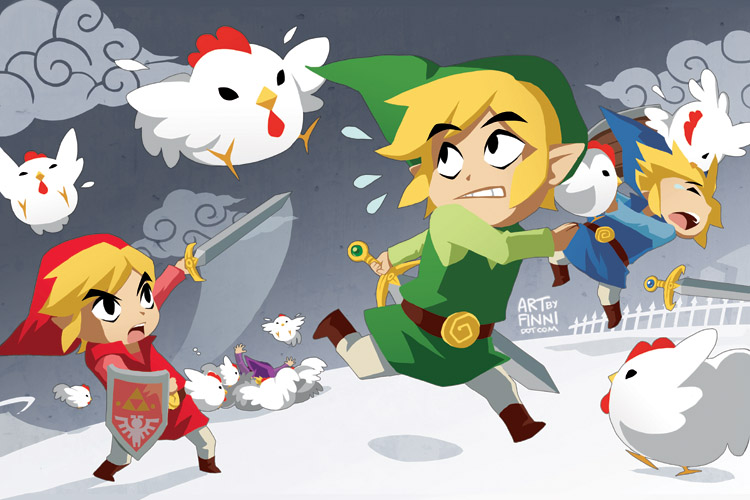
\includegraphics[width=0.6\textwidth]{figures/Sample/tumblr_static_eaceks0rfxsss8o4swscw40wo.jpg}
    \caption[Single Figure Environment Listed Title]{This is a single figure 
    environment}
    \label{fig_singleenv}
\end{figure}

This is a multi-image figure with a top (Figure~\ref{fig_multienv_1}) and bottom (Figure~\ref{fig_multienv_2}) aligned subfigures:

\begin{figure}[ht]
	\centering
	\begin{subfigure}[t]{\textwidth}
		\centering
		
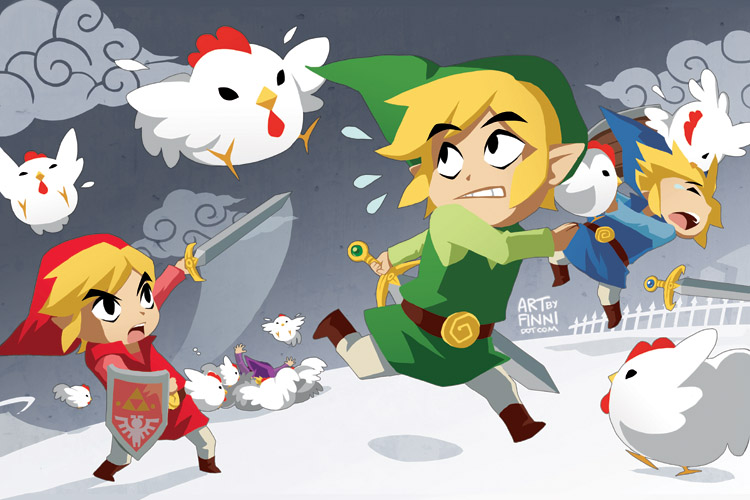
\includegraphics[width=0.7\textwidth]{figures/Sample/tumblr_static_eaceks0rfxsss8o4swscw40wo.jpg}
		\caption{Figure 1}
		\label{fig_multienv_1}
	\end{subfigure}
	~
	\begin{subfigure}[t]{\textwidth}
		\centering
		
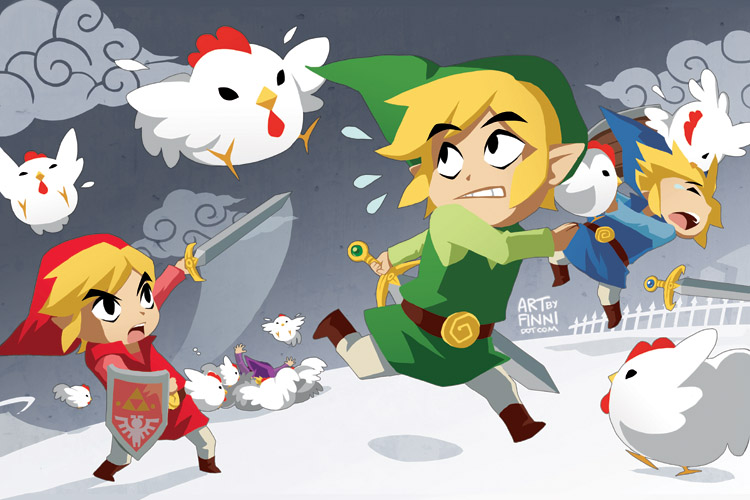
\includegraphics[width=0.7\textwidth]{figures/Sample/tumblr_static_eaceks0rfxsss8o4swscw40wo.jpg}
		\caption{Figure 2}
		\label{fig_multienv_2}
	\end{subfigure}
	
	\caption{A Multi-Figure Environment}
	\label{fig_multienv}
\end{figure}

\section{Tables}

Here is a sample table (Table~\ref{tab_sample}):

	\begin{table}[ht]
	\centering
	\begin{tabular}{ m{0.2\textwidth} m {0.1\textwidth} m{0.15\textwidth} }
		\toprule
		A & $\longleftrightarrow$ & B \\
		C & $\longleftrightarrow$ & D \\
		\bottomrule	
	\end{tabular}	
	\caption{A sample table}	
	\label{tab_sample}
\end{table}

\subsection{Long Tables}
A sample long table is shown in Appendix~\ref{appendix_b}.

\section{Equations}

Here is a sample equation (Equation~\ref{eq_lineslope}):

\begin{equation} \label{eq_lineslope}
	y = mx + b
\end{equation}                  
       \setcounter{figure}{0}
       \setcounter{equation}{0}
       \setcounter{table}{0}

  \chapter{Conclusion}
An ODE is a type, and it exists in many forms. Previously to this research, the Drasil Framework had no flexible and reusable structure for capturing ODE information. The Drasil teams have to manually extract useful information from the original ODE to instruct the Drasil Code Generator to generate code. This approach propagates duplicated information and loses traceability. The newly created structure, \verb|DifferentialModel|, stores linear ODE information based on the conventional matrix concept. It provides the flexibility to transform a linear ODE from one form to another mathematically equivalent form. Once we capture the knowledge of ODE in the new structure, we can reuse it for other purposes, such as producing the numerical solution and displaying the ODE.

Along with \verb|DifferentialModel|, four selected external libraries are responsible for producing the numerical solution for a system of first-order ODEs. Drasil users can get a numerical solution by choosing an algorithm. Currently, although the Calculations module outputs a finite stream of real numbers, $\mathbb{R}^m$, there are other design options. The C\# OSLO provides an option to output an infinite stream of real numbers, $\mathbb{R}^{\infty}$. It has richer data than $\mathbb{R}^m$. Also, outputting the ODE as a function that can return the value of the dependent variable for any value of the independent variable could help generate libraries in Drasil. We did not complete implementing the new specifications for this, but the analysis provides a starting point for future research.

\verb|DifferentialModel| provides reusable ODE information, and external libraries provide mathematical knowledge for solving the ODE. Before we bridge the gap between \verb|DifferentialModel| and external libraries, we enable solving any higher-order ODEs with manually written equations via external libraries. The Double Pendulum case study demonstrates the Drasil Framework can generate code that solves a system of higher-order non-linear ODEs. With all implementations, we are ready to bridge the gap by automating the process of extracting useful information from \verb|DifferentialModel| and then forming an \verb|ODEInfo|. While we are solving a single higher-order linear ODE, we generate it instead of manually writing \verb|ODEInfo|. The automation removes the duplicated information and potentially increases traceability.

This research accomplishes three main goals. Firstly, we capture the knowledge of ODE in a flexible and reusable structure. Secondly, we expand the Drasil capability to solve any higher-order ODEs with manually written equations. The last one is removing the duplicated information caused by the implementation of solving ODEs.

        \setcounter{figure}{0}
        \setcounter{equation}{0}
        \setcounter{table}{0}

\begin{appendix}
    \chapter{Your Appendix}
\label{appendix_a}

This appendix provides detailed explanations of various parts of DifferentialModel.

\section{Constructors of DifferentialModel}
\label{const_de}

% \begin{listing}[ht]
\begin{haskell1}
-- $K_d$ is qdDerivGain
-- $y_t$ is opProcessVariable
-- $K_p$ is qdPropGain
-- $r_t$ is qdSetPointTD
imPDRC :: DifferentialModel
imPDRC = makeASingleDE
	time
	opProcessVariable
	lhs
	rhs
	"imPDRC"
	(nounPhraseSP "Computation of the Process Variable as a function of time")
	EmptyS
	where 
	lhs = [exactDbl 1 `addRe` sy qdDerivGain $* (opProcessVariable $^^ 1)]
	$+ (exactDbl 1 $* (opProcessVariable $^^ 2))
	$+ (exactDbl 20 `addRe` sy qdPropGain $* (opProcessVariable $^^ 0))
	rhs = sy qdSetPointTD `mulRe` sy qdPropGain
\end{haskell1}
\captionof{listing}{Using input language for the example~\ref{eq_odeexmaple} in DifferentialModel}
% \label{code_scexinputl}
% \end{listing}

% \begin{listing}[ht]
\begin{haskell1}
imPDRC :: DifferentialModel
imPDRC = makeASystemDE
	time
	opProcessVariable
	coeffs = [[exactDbl 1, exactDbl 1 `addRe` sy qdDerivGain, exactDbl 20 `addRe` sy qdPropGain]]
	unknowns = [2, 1, 0]
	constants = [sy qdSetPointTD `mulRe` sy qdPropGain]
	"imPDRC"
	(nounPhraseSP "Computation of the Process Variable as a function of time")
	EmptyS
\end{haskell1}
\captionof{listing}{Explicitly set values for the example~\ref{eq_odeexmaple} in DifferentialModel}
% \label{code_scexmatrix}
% \end{listing}

\section{Numerical Solution Implementation}
\label{numsol}

% \begin{listing}[ht]
\begin{python1}
def func_y_t(K_d, K_p, r_t, t_sim, t_step):
    def f(t, y_t):
        return [y_t[1], -(1.0 + K_d) * y_t[1] + -(20.0 + K_p) * y_t[0] + r_t * K_p]
    
    r = scipy.integrate.ode(f)
    r.set_integrator("dopri5", atol=Constants.Constants.AbsTol, rtol=Constants.Constants.RelTol)
    r.set_initial_value([0.0, 0.0], 0.0)
    y_t = [[0.0, 0.0][0]]
    while r.successful() and r.t < t_sim:
        r.integrate(r.t + t_step)
        y_t.append(r.y[0])
    
    return y_t
\end{python1}
\captionof{listing}{Source code of solving PDController in Scipy}
% \label{code_pythonscipy}
% \end{listing}

In line 1, \verb|func_y_t| is a function output the numerical solution, and it is a list of numbers. In the line 2, the local function \verb|f| contains ODE. The line 3 shows local function return a list. Since we want to solve a system of ODE, the index one is the first ODE in this system, and the index two is the second ODE this system. By calling \verb|scipy.integrate.ode|, we pack ODE information in the generic interface. The line between 5 and 10, are procedure how to set configuration and collecting results. Theoretically, we can just return the \verb|r| in line 4 to present returning a function of ODE.

% \begin{listing}[ht]
\begin{java1}
public static ArrayList<Double> func_y_t(double K_d, double K_p, double r_t, double t_sim, double t_step) {
	ArrayList<Double> y_t;
	ODEStepHandler stepHandler = new ODEStepHandler();
	ODE ode = new ODE(K_p, K_d, r_t);
	double[] curr_vals = {0.0, 0.0};

	FirstOrderIntegrator it = new DormandPrince54Integrator(t_step, t_step, Constants.AbsTol, Constants.RelTol);
	it.addStepHandler(stepHandler);
	it.integrate(ode, 0.0, curr_vals, t_sim, curr_vals);
	y_t = stepHandler.y_t;

	return y_t;
}
\end{java1}
\captionof{listing}{A linear system of first-order representation in ACM}
% \label{code_javaacm}
% \end{listing}

% \begin{listing}
\begin{cplusplus1}
vector<double> func_y_t(double K_d, double K_p, double r_t, double t_sim, double t_step) {
	vector<double> y_t;
	ODE ode = ODE(K_p, K_d, r_t);
	vector<double> currVals{0.0, 0.0};
	Populate pop = Populate(y_t);
		
	boost::numeric::odeint::runge_kutta_dopri5<vector<double>> rk = boost::numeric::odeint::runge_kutta_dopri5<vector<double>>();
	auto stepper = boost::numeric::odeint::make_controlled(Constants::AbsTol, Constants::RelTol, rk);
	boost::numeric::odeint::integrate_const(stepper, ode, currVals, 0.0, t_sim, t_step, pop);
	
	return y_t;
}	
\end{cplusplus1}
\captionof{listing}{A linear system of first-order representation in ODEINT}
% \label{code_cplusplusodeint}
% \end{listing}

% \begin{listing}[ht]
\begin{csharp1}
public static List<double> func_y_t(double K_d, double K_p, double r_t, double t_sim, double t_step) {
	List<double> y_t;
	Func<double, Vector, Vector> f = (t, y_t_vec) => {
		return new Vector(y_t_vec[1], -(1.0 + K_d) * y_t_vec[1] + -(20.0 + K_p) * y_t_vec[0] + r_t * K_p);
	};
	Options opts = new Options();
	opts.AbsoluteTolerance = Constants.AbsTol;
	opts.RelativeTolerance = Constants.RelTol;
	
	Vector initv = new Vector(new double[] {0.0, 0.0});
	IEnumerable<SolPoint> sol = Ode.RK547M(0.0, initv, f, opts);
	IEnumerable<SolPoint> points = sol.SolveFromToStep(0.0, t_sim, t_step);
	y_t = new List<double> {};
	foreach (SolPoint sp in points) {
		y_t.Add(sp.X[0]);
	}
	
	return y_t;
}
\end{csharp1}
\captionof{listing}{Source code of solving PDController in OSLO}
% \label{code_csharposlo}
% \end{listing}


\section{Algorithm in External Libraries}
\label{alg_externallib}

\begin{table}[ht]
\begin{tabular}{ p{0.2\textwidth} p{0.7\textwidth} }
	\textbf{Name} & \textbf{Description} \\
	\toprule
	\verb|zvode| & Complex-valued Variable-coefficient Ordinary Differential Equation solver, with fixed-leading-coefficient implementation. It provides implicit Adams method (for non-stiff problems) and a method based on backward differentiation formulas (BDF) (for stiff problems).\\ \hline
	\verb|lsoda| & Real-valued Variable-coefficient Ordinary Differential Equation solver, with fixed-leading-coefficient implementation. It provides automatic method switching between implicit Adams method (for non-stiff problems) and a method based on backward differentiation formulas (BDF) (for stiff problems).\\ \hline
	\verb|dopri5| & This is an explicit runge-kutta method of order (4)5 due to Dormand \& Prince (with stepsize control and dense output).\\ \hline
	\verb|dop853| & This is an explicit runge-kutta method of order 8(5,3) due to Dormand \& Prince (with stepsize control and dense output).\\
	\bottomrule	
\end{tabular}	
\caption{Algorithm Options in Scipy~\citep{scipyfun}}	
\label{tab_algscipy}
\end{table}

\begin{table}[ht]
\begin{tabular}{ p{0.27\textwidth} p{0.7\textwidth} }
	\textbf{Name} & \textbf{Description} \\
	\toprule
	\verb|Euler| & This class implements a simple Euler integrator for Ordinary Differential Equations.\\ \hline
	\verb|Midpoint| & This class implements a second order Runge-Kutta integrator for Ordinary Differential Equations.\\ \hline
	\verb|Classical RungeKutta| & This class implements the classical fourth order Runge-Kutta integrator for Ordinary Differential Equations (it is the most often used Runge-Kutta method).\\ \hline
	\verb|Gill| & This class implements the Gill fourth order Runge-Kutta integrator for Ordinary Differential Equations.\\ \hline
	\verb|Luther| & This class implements the Luther sixth order Runge-Kutta integrator for Ordinary Differential Equations.\\ \hline
	\verb|Higham and Hall| & This class implements the 5(4) Higham and Hall integrator for Ordinary Differential Equations.\\ \hline
	\verb|DormandPrince 5(4)| & This class implements the 5(4) Dormand-Prince integrator for Ordinary Differential Equations.\\ \hline
	\verb|DormandPrince 8(5,3)| & This class implements the 8(5,3) Dormand-Prince integrator for Ordinary Differential Equations.\\ \hline
	\verb|Gragg-Bulirsch-Stoer| & This class implements a Gragg-Bulirsch-Stoer integrator for Ordinary Differential Equations.\\ \hline
	\verb|Adams-Bashforth| & This class implements explicit Adams-Bashforth integrators for Ordinary Differential Equations.\\ \hline
	\verb|Adams-Moulton| & This class implements implicit Adams-Moulton integrators for Ordinary Differential Equations.\\
	\bottomrule	
\end{tabular}	
\caption{Algorithm Options in Apache Commons Maths~\citep{apachefun}}	
\label{tab_algacm}
\end{table}

\begin{table}[ht]
\begin{tabular}{ p{0.4\textwidth} p{0.5\textwidth} }
	\textbf{Name} & \textbf{Description} \\
	\toprule
	\verb|euler| & Explicit Euler: Very simple, only for demonstrating purpose\\ \hline
	\verb|runge_kutta4| & Runge-Kutta 4: The classical Runge Kutta scheme, good general scheme without error control.\\ \hline
	\verb|runge_kutta_cash_karp54| & Cash-Karp: Good general scheme with error estimation.\\ \hline
	\verb|runge_kutta_dopri5| & Dormand-Prince 5: Standard method with error control and dense output.\\ \hline
	\verb|runge_kutta_fehlberg78| & Fehlberg 78: Good high order method with error estimation.\\ \hline

	\verb|adams_bashforth_moulton| & Adams-Bashforth-Moulton: Multi-step method with high performance.\\ \hline
	\verb|controlled_runge_kutta| & Controlled Error Stepper: Error control for the Runge-Kutta steppers.\\ \hline
	\verb|dense_output_runge_kutta| & Dense Output Stepper: Dense output for the Runge-Kutta steppers.\\ \hline
	\verb|bulirsch_stoer| & Bulirsch-Stoer: Stepper with step size, order control and dense output. Very good if high precision is required..\\ \hline
	\verb|implicit_euler| & Implicit Euler: Basic implicit routine.\\ \hline
	\verb|rosenbrock4| & Rosenbrock 4: Solver for stiff systems with error control and dense output.\\ \hline
	\verb|symplectic_euler| & Symplectic Euler: Basic symplectic solver for separable Hamiltonian system.\\ \hline
	\verb|symplectic_rkn_sb3a_mclachlan| & Symplectic RKN McLachlan: Symplectic solver for separable Hamiltonian system with order 6.\\
	\bottomrule	
\end{tabular}	
\caption{Algorithm Options in ODEINT~\citep{odeintfun}}	
\label{tab_algodeint}
\end{table}

\begin{table}[ht]
\begin{tabular}{ p{0.2\textwidth} p{0.7\textwidth} }
	\textbf{Name} & \textbf{Description} \\
	\toprule
	\verb|RK547M| & This method is most appropriate for solving non-stiff ODE systems. It is based on classical Runge-Kutta formulae with modifications for automatic error and step size control.\\ \hline
	\verb|GearBDF| & It is an implementation of the Gear back differentiation method, a multi-step implicit method for stiff ODE systems solving.\\
	\bottomrule	
\end{tabular}	
\caption{Algorithm Options in OSLO~\citep{oslofun}}	
\label{tab_algodeint}
\end{table}

        \setcounter{figure}{0}
        \setcounter{equation}{0}
        \setcounter{table}{0}

    \chapter{Long Tables}
\label{appendix_b}

This appendix demonstrates the use of a long table that spans multiple pages.

\begin{center}
\begin{longtable}{P{3cm}P{3cm}P{2.5cm}P{3.5cm}}
\toprule
\hline
\textbf{Col A} & \textbf{Col B} & \textbf{Col C} & \textbf{Col D} \\ \midrule

\endfirsthead
\multicolumn{4}{c}{\textit{Continued from previous page}} \\ \hline
\textbf{Col A} & \textbf{Col B} & \textbf{Col C} & \textbf{Col D} \\ \hline
\endhead
\hline \multicolumn{4}{r}{\textit{Continued on the next page}} \\
\endfoot
\hline
\endlastfoot

A & B & C & D \\ \midrule

A & B & C & D \\ \midrule

A & B & C & D \\ \midrule

A & B & C & D \\ \midrule

A & B & C & D \\ \midrule

A & B & C & D \\ \midrule

A & B & C & D \\ \midrule

A & B & C & D \\ \midrule

A & B & C & D \\ \midrule

A & B & C & D \\ \midrule

A & B & C & D \\ \midrule

A & B & C & D \\ \midrule

A & B & C & D \\ \midrule

A & B & C & D \\ \midrule

A & B & C & D \\ \midrule

A & B & C & D \\ \midrule

A & B & C & D \\ \midrule

A & B & C & D \\ \midrule

A & B & C & D \\ \midrule

A & B & C & D \\ \midrule

\hline
\end{longtable}
\end{center}

        \setcounter{figure}{0}
        \setcounter{equation}{0}
        \setcounter{table}{0}
\end{appendix}

% The bibliography is set up to allow for multiple bib files
\bibliographystyle{acm}
\bibliography{references,references_another}

\label{NumDocumentPages}

\end{document}
% ********************************
